\documentclass[adraft,creativecommons]{eptcs}
\usepackage[utf8]{inputenc}

\usepackage{underscore}

\usepackage[T1]{fontenc}
\usepackage{mathpartir}
\usepackage{amssymb}
\usepackage{amsmath}
\usepackage{braket}
\usepackage{color}
\usepackage{xspace}
\usepackage{cleveref}
\crefformat{section}{\S#2#1#3}

\usepackage{adjustbox}
\usepackage{tikz}
\usetikzlibrary{quantikz}

% From: https://tomhennigan.blogspot.com/2012/01/grouped-emails-in-latex-with-href-and.html
\newcommand{\mailtodomain}[1]{\href{mailto:#1}{\nolinkurl{#1}}}

\title{Quantum Hoare Type Theory}

\author{
Kartik Singhal
\institute{University of Chicago}
\email{\mailtodomain{ks@cs.uchicago.edu}}
}

\begin{document}

\maketitle

\section{Introduction}

\section{Background}

\section{Quantum Hoare Type Theory}

\subsection{Examples}

\subsubsection{Bell states}

Our simplest example involves creation of a Bell (or EPR) state which is one of the four maximally entangled quantum states of two qubits. Specifically, we will create a circuit (\cref{fig:bell00}) to produce the first Bell state which we will write in the mnemonic notation as $\ket{\beta_{00}} = (\ket{00}+\ket{11})/\sqrt{2}$.

\begin{figure}
    \centering
    % \begin{adjustbox}{width=0.4\textwidth}
    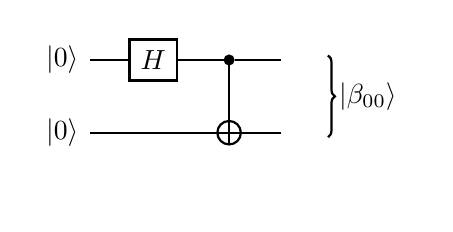
\begin{tikzpicture}
        \node[scale=1.0] {
            \begin{quantikz}
                \lstick{$\ket{0}$} & \gate{H} & \ctrl{1} & \qw & \midstick[2,brackets=left]{$\ket{\beta_{00}}$} \\
                \lstick{$\ket{0}$} & \qw & \targ{} & \qw & \\
            \end{quantikz}
        };
    \end{tikzpicture}
    % \end{adjustbox}
    \caption{Circuit to produce the first Bell state}
    \label{fig:bell00}
\end{figure}

\section{Discussion}

\section{Conclusion and perspectives}

\bibliographystyle{eptcsalpha}

\end{document}
